\include{template}
\cfoot{} %% if no page number is needed
\usepackage{setspace}
\usepackage{rotating}

\begin{document}

\begin{header}
Activité 4 -- Solutions aqueuses
\end{header}

\begin{enumerate}
\item Quand on prépare de l'eau salée :
\begin{multicols}{2}
\begin{enumerate}
\item l'eau est le solvant, le sel est le soluté ;
\item l'eau est le soluté, le sel est le solvant ;
\item le mélange est une solution aqueuse ;
\item on réalise une dilution ;
\item on réalise une dissolution ;
\item on réalise une distillation. 
\end{enumerate}
\end{multicols}

\item Quand on ajoute de l'eau à du sirop pour se désaltérer :
\begin{multicols}{2}
\begin{enumerate}
\item le sucre est un soluté ;
\item le sucre est un solvant ;
\item on réalise une dissolution ;
\item on réalise une dilution ;
\item la concentration en sucre dans la solution finale est plus élevée que dans le sirop.
\end{enumerate}
\end{multicols}

\item On dissout de l'aspirine dans de l'eau selon les trois situations ci-dessous.
\begin{multicols}{2}
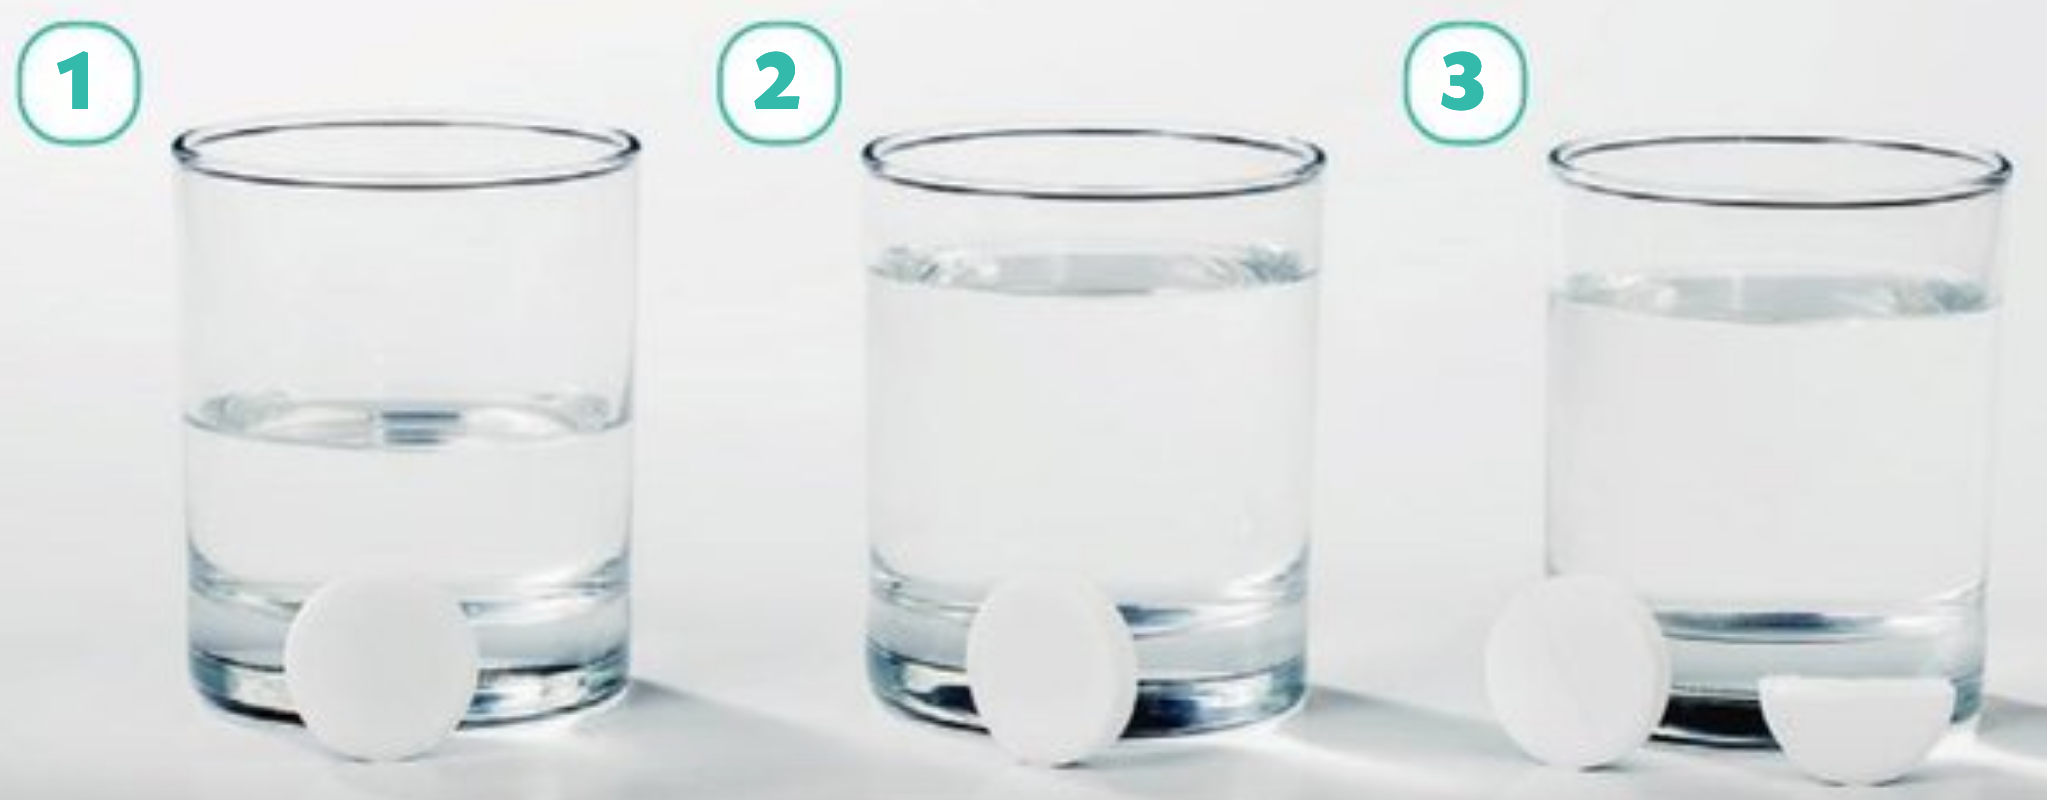
\includegraphics[scale=0.21]{images/exo10p43.png}

\begin{spacing}{1.5}
Compléter la phrase suivante :

\og La solution numéro \underline{\quad} est plus concentrée que la solution \underline{\quad}, elle même plus concentrée que la solution \underline{\quad}.\fg{}
\end{spacing}
\end{multicols}

\item Sur une étiquette d'eau minérale, on lit \og Ca\textsuperscript{2+} : 166 mg/L \fg{}.
Il s'agit de :
\begin{multicols}{2}
\begin{enumerate}
\item la masse volumique des ions calcium ;
\item la concentration massique en ions calcium ;
\item la teneur en ions calcium ;
\item du titre massique en ions calcium.
\end{enumerate}
\end{multicols}

\item Une solution aqueuse de sulfate de cuivre est saturée si :
\begin{multicols}{2}
\begin{enumerate}
\item on ne peut plus dissoudre de solvant ;
\item on ne peut plus dissoudre de soluté ;
\item il y a autant de soluté que de solvant ; 
\end{enumerate}
\end{multicols}

\item La solubilité en masse d'une espèce chimique :
\begin{multicols}{2}
\begin{enumerate}
\item est la masse maximale de soluté pouvant être dissout dans un litre de solution ;
%\item peut s'exprimer en g/L ;
%\item peut s'exprimer en g\cdot L\textsuperscript{-1} ;
%\item peut s'exprimer en g/L\textsuperscript{-1} ;
\item est la concentration maximale en une espèce chimique qu'il est possible d'obtenir en solution ;
\item est la masse maximale de solvant pouvant être dissout dans un litre de une solution ;
\item dépend de la température ;
\item dépend du solvant ;
\item dépend du soluté.
\end{enumerate}
\end{multicols}

\item Isoler la grandeur en bleu dans chacune des expressions suivantes :
\begin{multicols}{4}
\begin{enumerate}
\item $C_\mathrm{m} = \dfrac{\textcolor{bleu_f}{m}}{V}$ ;
\item $C_\mathrm{m} = \dfrac{m}{\textcolor{bleu_f}{V}}$ ;
\item $m = \textcolor{bleu_f}{t} \times V$ ;
\item $t_\mathrm{m}\times \textcolor{bleu_f}{V_\mathrm{m}} =  t_\mathrm{f}\times V_\mathrm{f}$.
\end{enumerate}
\end{multicols}


\flushright
\footnotesize
\begin{turn}{180}
Réponses :
(a) $\textcolor{bleu_f}{m} = C_\mathrm{m} \times V$ ; (b) $\textcolor{bleu_f}{V} = \dfrac{m}{C_\mathrm{m}} $ ; (c) $\textcolor{bleu_f}{t} = \dfrac{m_\mathrm{max}}{V}$ ; (d) $\textcolor{bleu_f}{V_\mathrm{m}} = \dfrac{t_\mathrm{f}\times V_\mathrm{f}}{t_\mathrm{m}}$.
\hfill
\end{turn}

\end{enumerate}

\end{document}